%************************************************
\chapter{A Proof System}\label{ch:system} % $\mathbb{ZNR}$
%************************************************

\section{A Proof System}
In this section we study the necessary liberal precondition: 
$$wlp.C.F\implies G$$


\section{Sketches} 
\note{In this section are informal sketches of my thoughts.}

\paragraph{Possible ways to approach this}\ 

\textbf{1.} $wlp.C.F \Longrightarrow G $ but restrict G by requiring that the postcondition F is always reachable. 
Effectively this transfers wlp in demonic setting to wlp in angelic setting, the postcondition being ``guaranteed'' changes into ``reachable''. 
Remember: both Dijkstra's wp and wlp are in demonic setting, and they are related by $wp_d.C.X = wp_d.C.true \wedge wlp_d.C.X$. 
Explore the relationship between $wp_angelic$, $wp_demonic$, $wlp_angelic$, $wlp_demonic$? 
Then the results in \cite{zhang22} and \cite{dijkstra90} can be linked. 
But then who uses angelic wlp? 
Also, does it even make sense to investigate this, since they are both extrema, specially in a quantitative setting. 

\textbf{2.}$$wlp.C.F \Longrightarrow G \equiv \neg G \Longrightarrow \neg wlp.C.F \equiv \neg G \Longrightarrow  wp.C.\neg F $$ 
This corresponds to total correctness, but negatively. 
\hoare{\neg G}{C}{\neg F} would be a valid Hoare Triple. 
But negative is not pretty. 

\begin{figure}[ht!]\centering
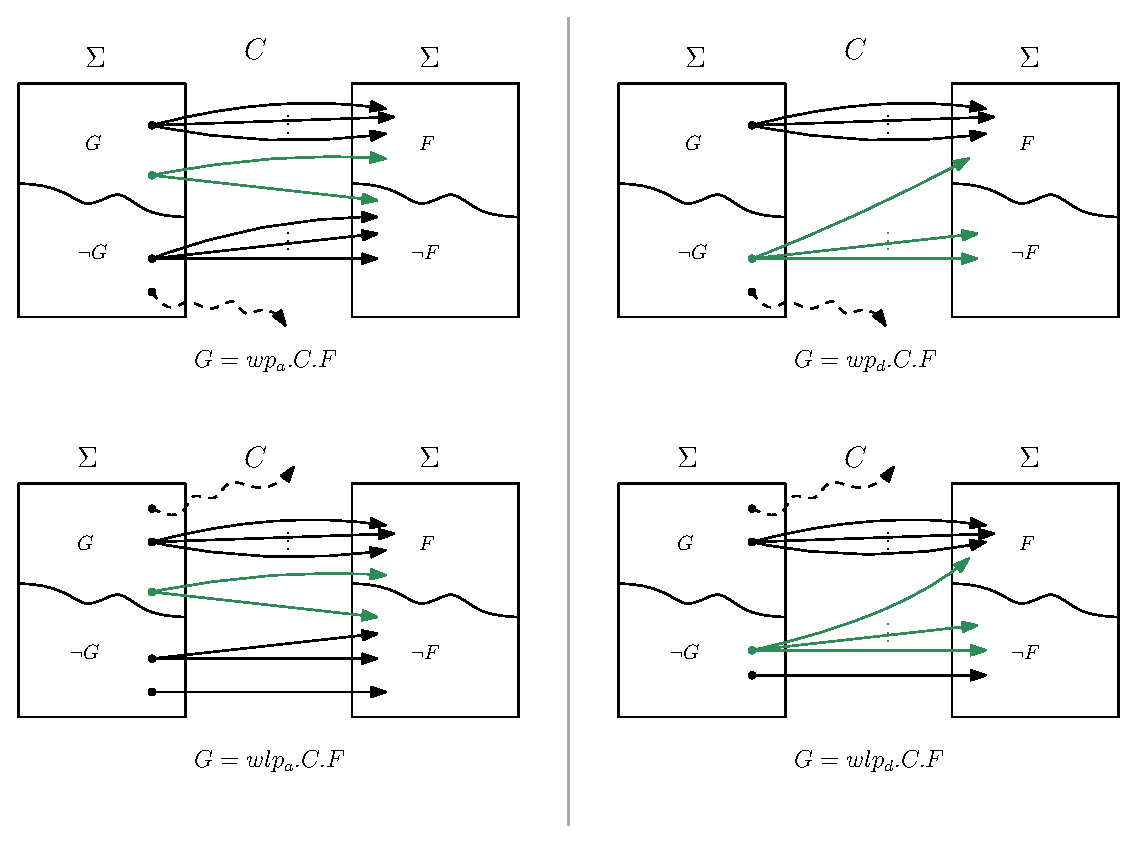
\includegraphics[width=\textwidth]{image/wp-wlp-angelic-demonic.eps}
\caption{Angelic and Demonic Nondeterminism}
\label{fig:ang-dem}
\end{figure}


\begin{figure}[ht!]\centering
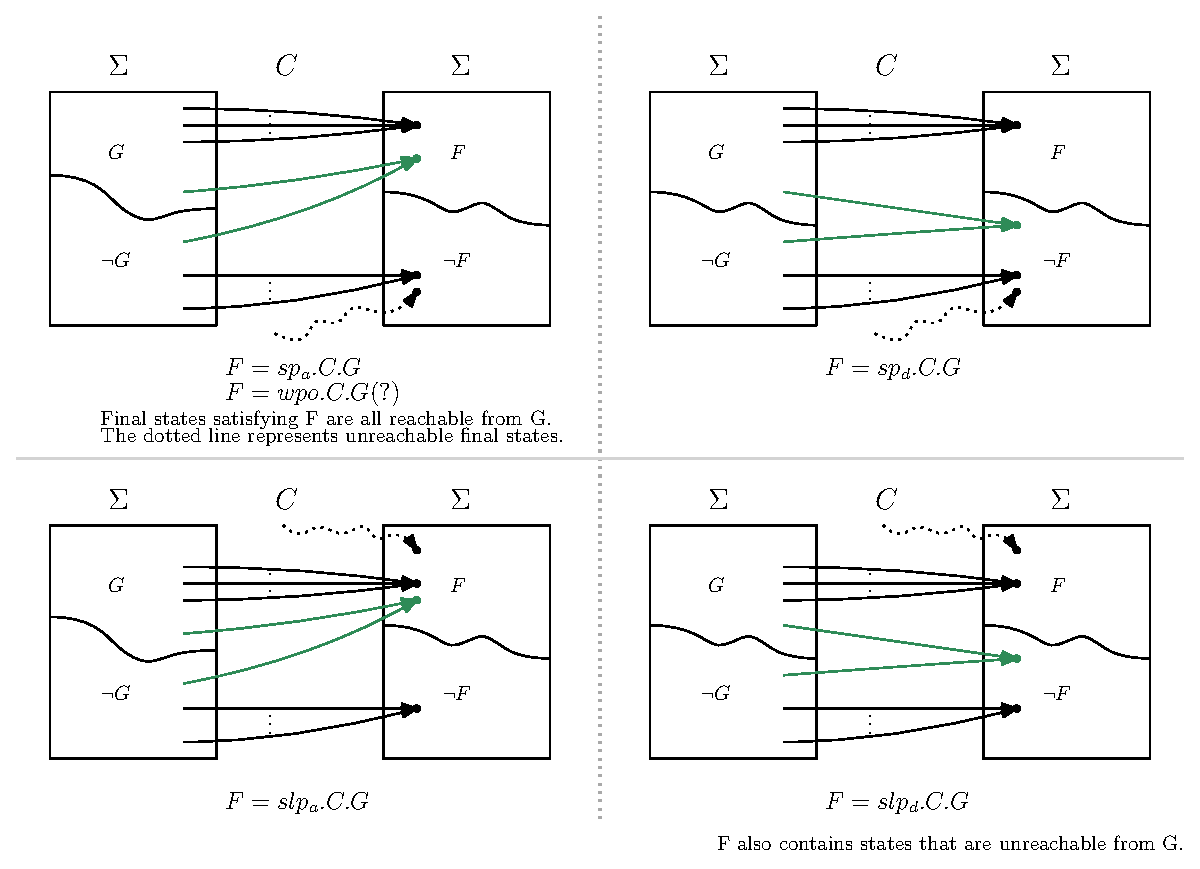
\includegraphics[width=\textwidth]{image/sp-slp.eps}
\caption{sp and slp}
\label{fig:sp-slp}
\end{figure}


\begin{figure}[ht!]\centering
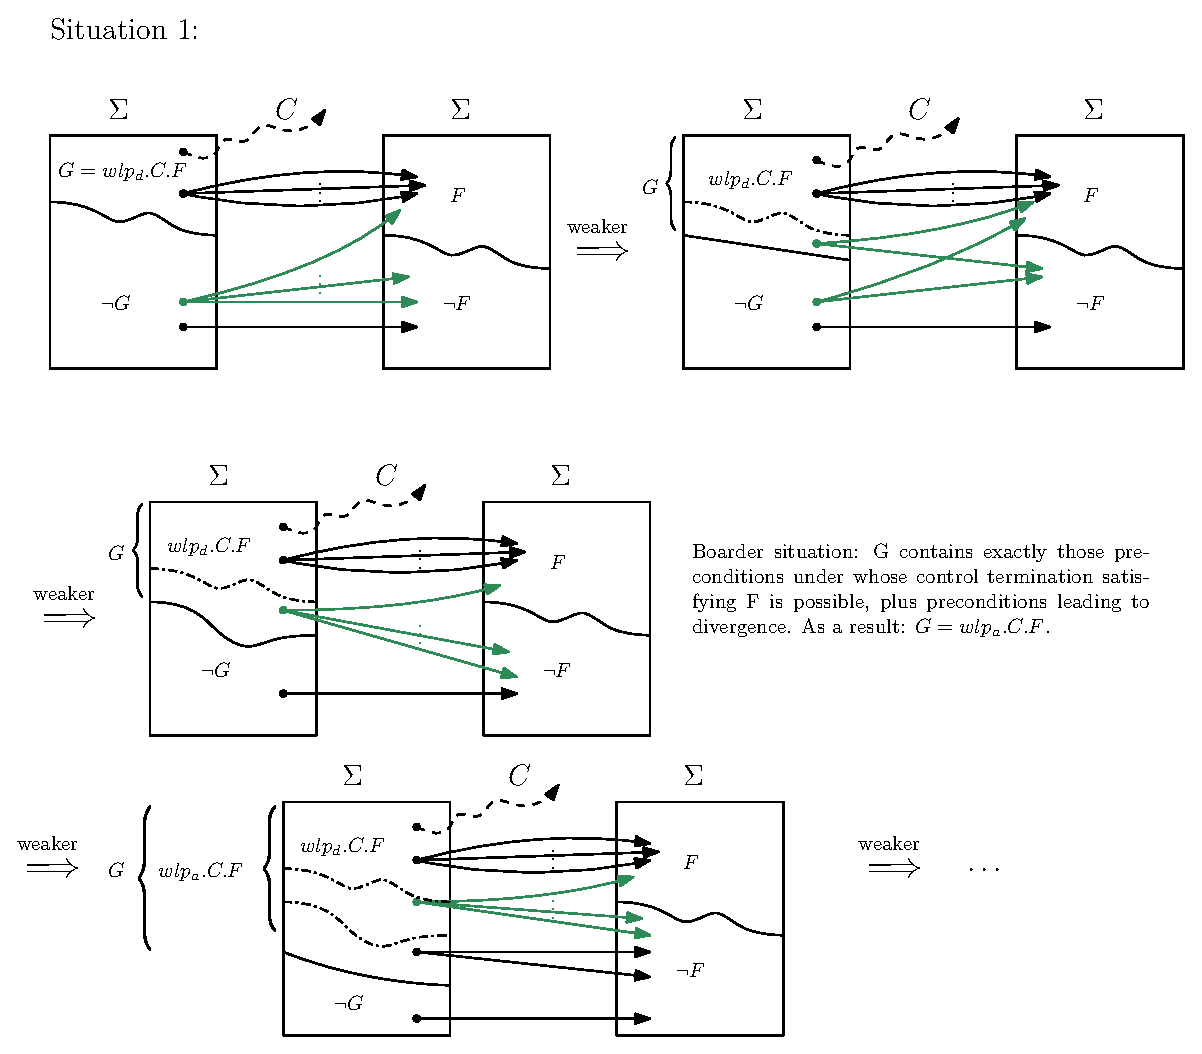
\includegraphics[width=\textwidth]{image/wlp-g-1.eps}
\caption{When wlp implies G - situation 1}
\label{fig:wlp-g-1}
\end{figure}

\begin{figure}[ht!]\centering
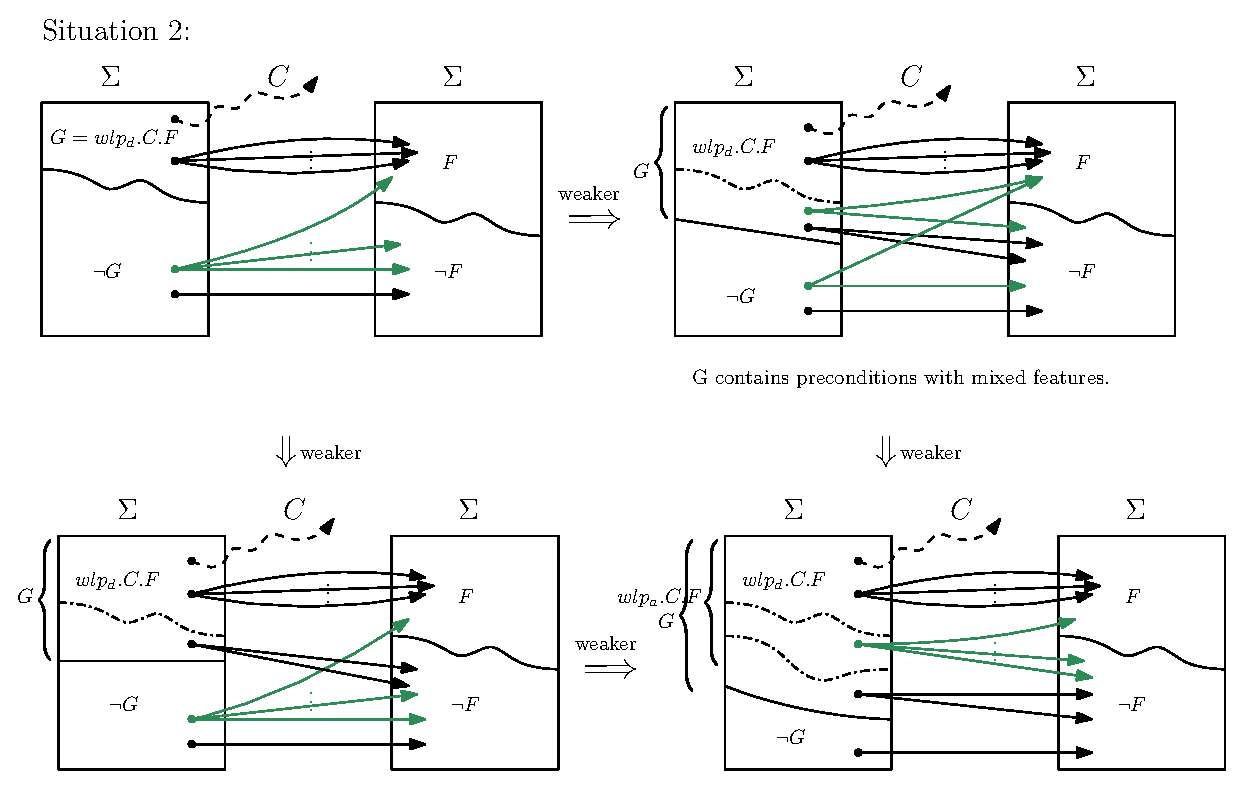
\includegraphics[width=\textwidth]{image/wlp-g-2.eps}
\caption{When wlp implies G - situation 2}
\label{fig:wlp-g-2}
\end{figure}


%*****************************************
%*****************************************
%*****************************************
%*****************************************
%*****************************************
